\chapter{Prompt Optimisation as an Adaptive Mechanism}
\label{chap:prompt-optimisation}

\section{Motivation and problem statement}
\label{sec:motivation-prompt-adaptation}

Under the alert rule in Chapter~\ref{ch:drift} (Section~\ref{sec:mcnemar-section}), statistically supported degradation is evidence of changed deployment behaviour on $\mathcal{D}_n$ while labels and task specification are fixed. Fine-tuning the provider model is excluded here (API-only access; cost). The controllable input is the prompt $\pi$.

Let the deployed classifier at time $t$ be
\begin{equation}
    f_t(x;\pi) = f(x;\pi,\theta_t),
\end{equation}
with prompt $\pi$ and provider-controlled state $\theta_t$. Drift in $\theta_t$ may occur with fixed $\pi$. Prompt optimisation seeks $\pi^\star$ that restores or improves predictive quality on a labelled optimisation set without changing the API model identifier, when such recovery is preferable to immediate fallback to another $m\in\mathcal{M}_{\mathrm{cand}}$.

\section{Automatic prompt optimisation}
\label{sec:general-formulation-apo}

Let $\mathcal{P}$ denote admissible prompts, $\mathcal{D}_{\mathrm{opt}}=\{(x_i,y_i)\}_{i=1}^n$ the optimisation dataset, and fix $m \in \mathcal{M}_{\mathrm{cand}}$ (typically $m_{\mathrm{curr}}$). Provider variation enters through $\theta_t$ in $f_t(x;\pi)=f(x;\pi,\theta_t)$. For $\pi \in \mathcal{P}$,
\begin{equation}
    J_t(\pi)
    =
    \frac{1}{n}\sum_{i=1}^{n}
    \ell\!\left(f_t(x_i;\pi),y_i\right).
\end{equation}
For binary classification, $\ell(f_t(x_i;\pi),y_i)=\mathbb{I}(f_t(x_i;\pi)=y_i)$ and $J_t(\pi)$ is empirical accuracy on $\mathcal{D}_{\mathrm{opt}}$. The APO problem is
\begin{equation}
    \pi_t^\star
    \in
    \arg\max_{\pi \in \mathcal{P}} J_t(\pi).
\end{equation}

The search space $\mathcal{P}$ is discrete; objectives are black-box (outputs only); each candidate requires repeated API calls. Practical methods approximate $\arg\max$ by iterative \emph{generate--evaluate--update} schemes. Let $\mathcal{C}_k$ be candidates at iteration $k$, $\mathcal{E}_k=\mathrm{Eval}(\mathcal{C}_k,\mathcal{D}_{\mathrm{opt}})$ feedback, and $\mathcal{U}$ an update rule:
\begin{align}
    \mathcal{C}_0 &= \mathrm{Init}(\mathcal{D}_{\mathrm{opt}}), \\
    \mathcal{E}_k &= \mathrm{Eval}(\mathcal{C}_k,\mathcal{D}_{\mathrm{opt}}), \\
    \mathcal{C}_{k+1} &= \mathcal{U}(\mathcal{C}_k,\mathcal{E}_k),
\end{align}
with final selection $\pi^\star \in \arg\max_{\pi \in \mathcal{C}_K} J_t(\pi)$. Feedback may reduce to scores $\mathcal{E}_k = \{J_t(\pi) : \pi \in \mathcal{C}_k\}$ or add errors, traces, and textual critiques.

\begin{figure}[ht]
\centering
\fbox{
\parbox{0.92\linewidth}{
\centering
Seed prompt(s) $\rightarrow$ Candidate generation $\rightarrow$ Evaluation on $\mathcal{D}_{\mathrm{opt}}$ $\rightarrow$ Selection / filtering $\rightarrow$ Updated prompt(s)
}}
\caption{Generic APO loop; implementations differ in $\mathrm{Init}$, $\mathrm{Eval}$, and $\mathcal{U}$.}
\label{fig:apo-generic-loop}
\end{figure}

\section{Method families and API feasibility}
\label{sec:taxonomy-apo}

\begin{figure}[ht]
    \centering
    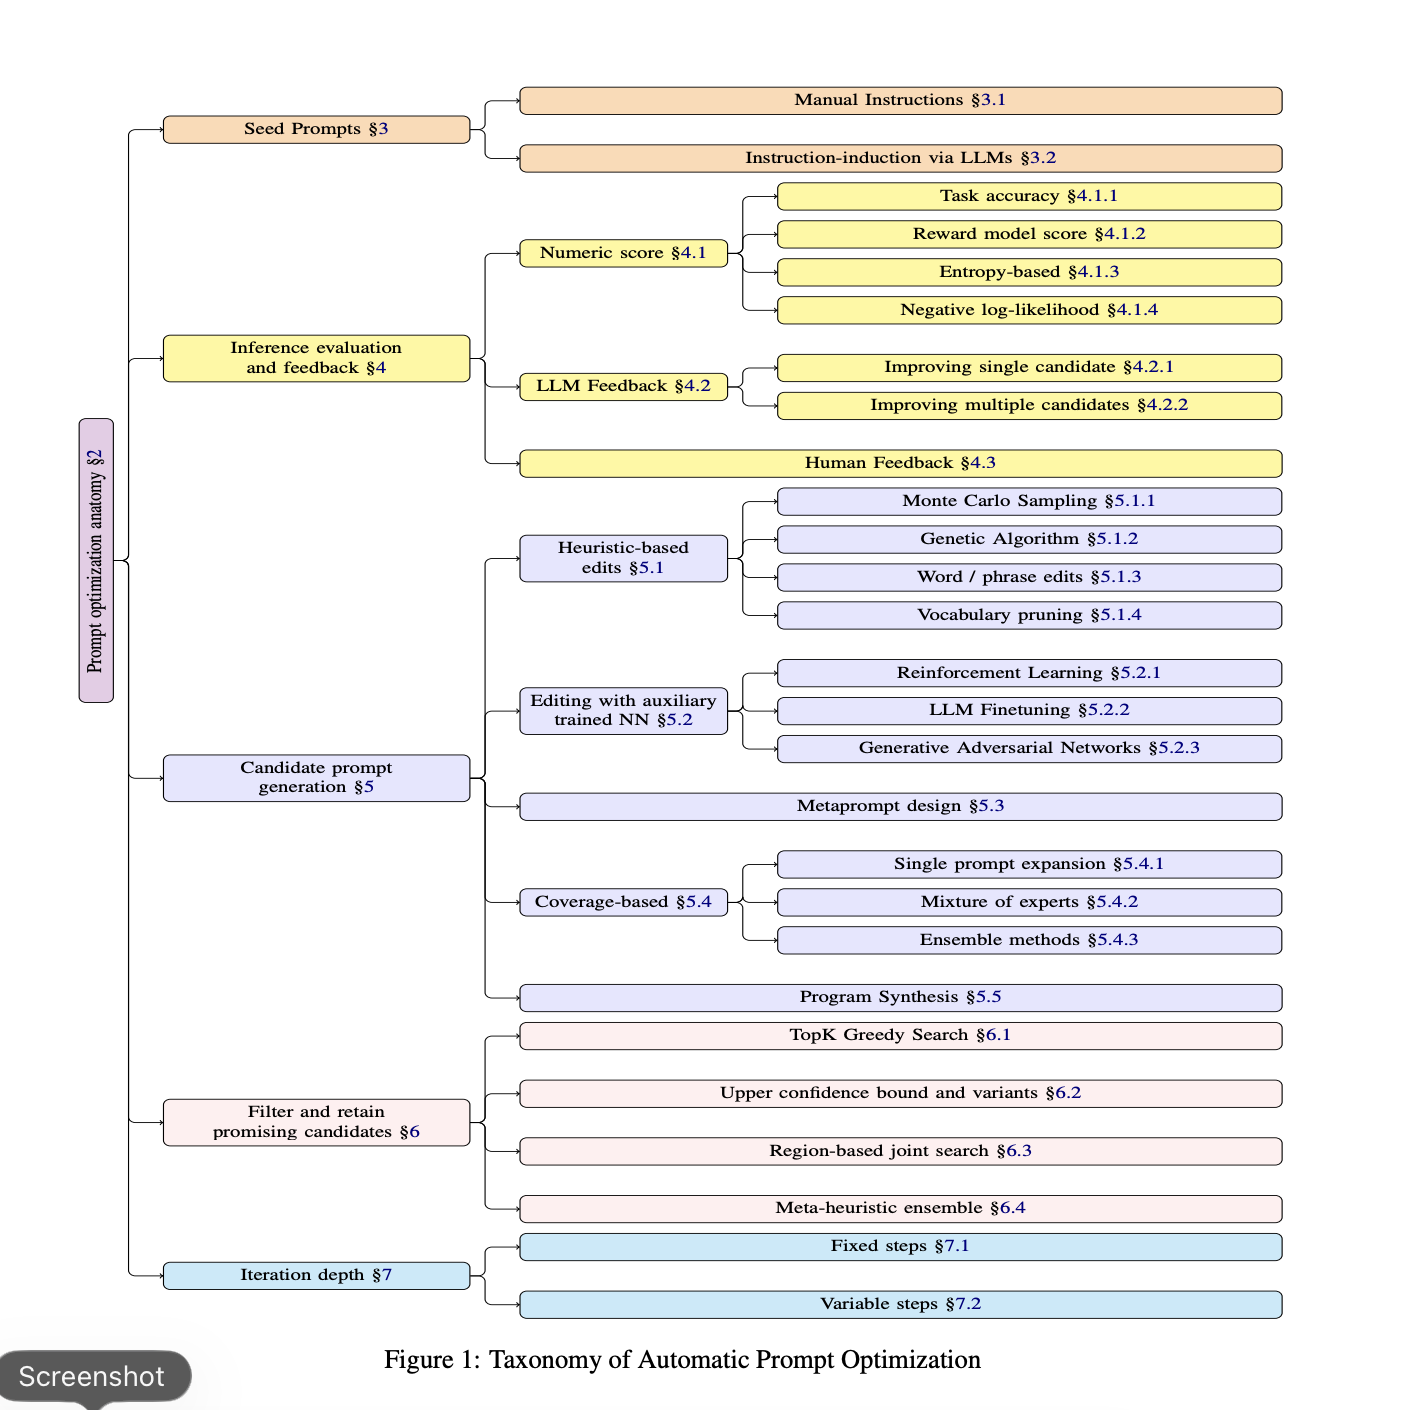
\includegraphics[width=\linewidth]{assets/Screenshot 2026-03-16 at 12.25.23.png}
    \caption{Taxonomy of automatic prompt optimisation methods~\cite{ramnath2025survey}.}
    \label{fig:apo-taxonomy}
\end{figure}

Survey work organises APO into a common pipeline (seed, generate, evaluate, filter, iterate)~\cite{ramnath2025survey}. For LLM-as-a-Service, gradient-based and soft-prompt methods~\cite{lester2021prompt,li2021prefix,shin2020autoprompt} are largely excluded: they require gradients or internal access. Reinforcement-learning prompt search~\cite{deng2022rlprompt} is black-box compatible but often sample-expensive under API budgets. LLM-as-optimizer methods (APE, ProTeGi, OPRO)~\cite{zhou2022ape,pryzant2023protegi,yang2024opro} rewrite prompts from feedback; many behave as greedy local search and can induce regressions on previously correct instances. Evolutionary approaches maintain populations and explore discrete non-convex spaces~\cite{guo2024evoprompt,fernando2024promptbreeder}. Bayesian and program-level optimisers (e.g.\ MIPROv2)~\cite{opsahlong2024mipro} target structured pipelines and aggregate scores; they are less aligned with instance-level retention of diverse behaviours when regressions must be controlled.

\section{GEPA}
\label{sec:gepa}

This work uses GEPA (Genetic--Pareto Evolutionary Prompt Optimisation)~\cite{agrawal2025gepa}: black-box evaluation only, evolutionary pools, reflective mutation by a language model, and Pareto-based retention over instances.

\subsection{Algorithm}

GEPA maintains a pool of candidates, initially the base configuration $\Phi$. Data are split into a feedback set $D_{\mathrm{feedback}}$ and a validation set $D_{\mathrm{pareto}}$; optimisation runs until a rollout budget is exhausted. At iteration $k$: (i)~sample a parent from the Pareto-filtered pool; (ii)~select a module (e.g.\ round-robin); (iii)~run a minibatch rollout on $D_{\mathrm{feedback}}$; (iv)~a reflection model proposes an updated prompt from traces and feedback; (v)~accept if minibatch score improves, then evaluate on $D_{\mathrm{pareto}}$. The returned candidate maximises aggregate score on $D_{\mathrm{pareto}}$. GEPA+Merge adds crossover between lineages. The method is designed for sample-efficient adaptation relative to alternatives such as GRPO in the original experiments~\cite{agrawal2025gepa}.

\subsection{Formalisation on \texorpdfstring{$\mathcal{D}_{\mathrm{opt}}$}{D\_opt}}
\label{sec:formal-gepa}

Let $\mathcal{D}_{\mathrm{opt}} = \{(x_1,y_1),\dots,(x_n,y_n)\}$ coincide with the disagreement-based monitoring material or a training split thereof. For prompt $\pi$, define per-instance correctness
\begin{equation}
    s_i(\pi)=\mathbb{I}\!\left(f_t(x_i;\pi)=y_i\right),
    \qquad
    \mathbf{s}(\pi)=(s_1(\pi),\dots,s_n(\pi))\in\{0,1\}^n.
\end{equation}

\begin{definition}[Pareto dominance]
$\pi^{(A)} \succ \pi^{(B)}$ if $s_i(\pi^{(A)}) \ge s_i(\pi^{(B)})$ for all $i$ and $s_j(\pi^{(A)}) > s_j(\pi^{(B)})$ for at least one $j$.
\end{definition}

Let $\mathcal{C}_k$ be the candidate set after $k$ updates. Non-dominated candidates are
\begin{equation}
    \mathcal{F}_k
    =
    \left\{
        \pi \in \mathcal{C}_k
        \;\middle|\;
        \nexists \tilde{\pi} \in \mathcal{C}_k \text{ such that } \tilde{\pi} \succ \pi
    \right\}.
\end{equation}
Reflective mutation maps a parent $\pi_k$, traces $\mathcal{T}_k$, and textual feedback $\mathcal{F}_k^{\mathrm{text}}$ to an offspring via $\pi_k' = \mathcal{M}_{\mathrm{refl}}(\pi_k,\mathcal{T}_k,\mathcal{F}_k^{\mathrm{text}})$. Pool update uses Pareto retention:
\begin{equation}
    \mathrm{ParetoRetain}(\mathcal{A})
    =
    \left\{
        \pi \in \mathcal{A}
        \;\middle|\;
        \nexists \pi' \in \mathcal{A} \text{ with } \pi' \succ \pi
    \right\}.
\end{equation}

\paragraph{Regression and recovery.}
For deployed prompt $\pi_0$ and candidate $\pi$, align with paired flips in Chapter~\ref{ch:drift}:
\begin{equation}
    R_{\mathrm{new}}(\pi \mid \pi_0)
    =
    \sum_{i=1}^n
    \mathbb{I}\bigl(s_i(\pi_0)=1,\; s_i(\pi)=0\bigr),
    \qquad
    G_{\mathrm{fix}}(\pi \mid \pi_0)
    =
    \sum_{i=1}^n
    \mathbb{I}\bigl(s_i(\pi_0)=0,\; s_i(\pi)=1\bigr).
\end{equation}
Scalar $J_t(\pi)=\frac{1}{n}\sum_i s_i(\pi)$ tracks only $G_{\mathrm{fix}}-R_{\mathrm{new}}$; Pareto retention keeps candidates that trade off instances differently, which matters when limiting $R_{\mathrm{new}}$ is as important as increasing $G_{\mathrm{fix}}$ on the disagreement-heavy subset (Chapter~\ref{ch:data}).

\paragraph{Fit to this thesis.}
GEPA requires no gradients or weights; it matches API-only deployment. Repeated drift events favour bounded rollout cost. The monitoring subset emphasises boundary cases where small prompt edits can flip labels; maintaining a frontier of non-dominated candidates mitigates single-trajectory greedy overfitting.

Prompt optimisation is invoked only after an alert under Chapter~\ref{ch:drift}. Recovered prompts are re-evaluated on $\mathcal{D}_n$ with the same metrics and cost comparison as in Section~\ref{sec:model-comparison-manual}; the implementation loop is documented in Chapter~\ref{chap:system-architecture}.
